%!TEX root = ../main.tex

\section{Stability analysis of the equilibrium solutions}
\label{sec:theoretical_analysis}

Under certain conditions the electrical breakdown can develop
form small perturbations of the properties of the undamaged medium.
To clarify these conditions in this section we study
stability of the constant solutions~$\phi(x, t) \equiv C = \text{const}$, $C \in [0, 1]$
of the equation~\eqref{eq:one_dim}.

First, one have to find stationary constant solutions of~\eqref{eq:one_dim}.
From definition~\eqref{eq:epsilon} it follows the following expression for derivatives
of~$\epsilon(\phi)$:
\begin{equation}
	\epsilon'(\phi) = \cfrac{-\epsilon_0 f'(\phi)}{(f(\phi) + \delta)^2} \tsemicolon \qquad \epsilon''(\phi) = \epsilon_0 \cfrac{2 (f'(\phi))^2 - f''(\phi)(f(\phi) + \delta)}{(f(\phi) + \delta)^3} \tpoint
	\label{eq:epsilon_derivatives}
\end{equation}

Substituting~$\phi(x, t) \equiv C$ into~\eqref{eq:one_dim} and
taking~\eqref{eq:epsilon_derivatives} into account, one have:
\begin{equation}
	f'(C) \left( \cfrac{\Gamma}{l^2} - \half K_\Phi^2 \cfrac{\epsilon_0}{(f(C) + \delta)^2} \right) = 0 \tpoint
	\label{eq:equilibrium}
\end{equation}
First, consider the case~$f'(C) = 12C^2 (1 - C) = 0$
which leads to~$C = 0,1$. Hence, $\phi \equiv 0$ и $\phi \equiv 1$ are
equilibrium solutions.

Second, let~$C \neq 0, 1$. Then
\[
\cfrac{\Gamma}{l^2} = \cfrac{K_\Phi^2 \epsilon_0}{2 (f(C) + \delta)^2}
\quad \text{and} \quad
f(C) + \delta = K_\Phi l \sqrt{\cfrac{\epsilon_0}{2 \Gamma}}.
\]

Note that~$f(C) \in [0, 1]$, and, moreover, $f(\phi)$ is monotonically
increasing. Therefore, under condition $K_\Phi l \sqrt{\epsilon_0 / (2
  \Gamma)} \in (\delta, 1 + \delta)$,
equation~\eqref{eq:equilibrium} has solution $C_3\ne 0,1$ given by
\begin{equation}
	C_3 = f^{-1} \left( K_\Phi l \sqrt{\cfrac{\epsilon_0}{2 \Gamma}} - \delta \right) \tpoint
	\label{eq:equilibrium_third}
\end{equation}
Otherwise equation~\eqref{eq:equilibrium} has only two solutions.

So, a number of constant equilibrium solutions depends on the satisfiability
of the condition
\begin{equation}
	\delta^2 < \cfrac{K_\Phi^2 l^2 \epsilon_0}{2 \Gamma} < (1 + \delta)^2 \tpoint
	\label{cond:equilibriums_number}
\end{equation}
In what further it will be shown how the
condition~\eqref{cond:equilibriums_number} is connected to the
stability properties of the equilibrium solutions and
equation~\eqref{eq:one_dim} itself.

Let us turn now to the stability analysis of the equilibrium solutions.

Let~$\phi(x, t)$ be a solution of~\eqref{eq:one_dim}, $\delta \phi(x,
t)$ be its perturbation.
Writing down equation~\eqref{eq:one_dim} for perturbed solution~$\phi
+ \delta \phi$,
after linearization one arrives to the following equation for~$\delta\phi$:
\begin{equation}
  \cfrac{1}{m} \partt{(\delta \phi)} = \left(\half K_\Phi^2 \epsilon''(\phi) + \cfrac{\Gamma}{l^2} f''(\phi) \right) \delta \phi + \half \Gamma \partxx{(\delta \phi)} \tpoint
  \label{eq:variation}
\end{equation}
For further analysis it is convenient to write~\eqref{eq:variation} as
%
\begin{equation}
  \partt{(\delta \phi)} = A \delta \phi + B \partxx{(\delta \phi)} \tcomma
  \label{eq:variation_common}
\end{equation}
where~$A$ and~$B  > 0$ are the respective parameters.

Choosing~$\delta \phi = e^{\alpha t} \sin(\omega x)$, one obtains from~\eqref{eq:variation_common}
the following relation for parameters of the perturbation:
$$\alpha e^{\alpha t} \sin(\omega x) = A e^{\alpha t} \sin(\omega x) - B \omega^2 e^{\alpha t} \sin(\omega x) \tcomma$$
from where it follows that:
\begin{equation}
  \alpha = A - B \omega^2 \tpoint
  \label{eq:exponent_coefficient}
\end{equation}

% Summing up, let us combine now the three parts of the reasoning.
% Consider equilibrium solution~$\phi \equiv C$ of the
% equation~\eqref{eq:one_dim} perturbed by~$\delta \phi$.

% ; применим к $\delta \phi$ уравнение \eqref{eq:variation}, в
% $\epsilon''$ и $f''$ подставим $\phi = C$. Полученное уравнение
% имеет вид~\eqref{eq:variation_common}.

Now it is easy to see, that depending on the value of the coefficient
$$A = \half K_\Phi^2 \epsilon''(C) + \cfrac{\Gamma}{l^2} f''(C)$$
three cases arise:
%
\begin{enumerate}[label=\arabic*.]
\item $A > 0$. In this case from~$\omega^2 \in [0, A / B)$ it follows
  that~$\alpha > 0$, i.e., there exists perturbation~$\delta \phi$
  which grows in time. Hence, equilibrium solution~$\phi \equiv C$ is
  unstable in this case.
  
\item $A < 0$. Then for an arbitrary~$\omega$ it holds~$\alpha
  \leqslant A < 0$. Next, any perturbation~$\delta \phi$ on the
  interval~$[0, W]_x$ 
  can be represented as Fourier integral over harmonics which decreases
  not slower then harmonic for~$\omega = 0$.
  Hence, equilibrium solution~$\phi \equiv C$ is stable.
  
\item $A = 0$. Repeating the same reasoning as for the case~$A < 0$,
  one can observe that there exist arbitrarily slowly decreasing
  harmonics (i.e., harmonics with arbitrarily small~$\alpha$).
  This case correspond to neutral stability of the equilibrium
  solution and linear analysis does not provide any additional
  information.
  This case will considered in more details in what further.
\end{enumerate}

We now turn to the discussion of the particular equilibrium states.

Consider equilibrium solution~$\phi \equiv 0$.
One has~$f''(0) = 0$, $\epsilon''(0) = 0$
(see~\eqref{eq:epsilon_derivatives})
which leads to~$A = 0$.
As it was noted, this case requires for elaborate analysis which will be
performed later.

Consider equilibrium solution~$\phi \equiv 1$.
In this case~$f''(0) = -12$, $\epsilon''(0) = 12 \epsilon_0 / (1 +
\delta)^2$ (see~\eqref{eq:epsilon_derivatives}).
As a result, one arrives to
$$A = \half K_\Phi^2 \epsilon''(C) + \cfrac{\Gamma}{l^2} f''(C) = \cfrac{6 K_\Phi^2 \epsilon_0}{(1 + \delta)^2} - \cfrac{12 \Gamma}{l^2} \tpoint$$
The equilibrium state is stable under condition~$A < 0$, i.e., as 
\begin{equation}
  \cfrac{K_\Phi^2 l^2 \epsilon_0}{2 \Gamma} < (1 + \delta)^2 
  \label{cond:equilibrium_1_stable}
\end{equation}
holds.      
Lets find~$\omega_0$ for which, in the case if the unstable solution,
increasing harmonics are replaced by the decreasing ones.
To do this, consider~\eqref{eq:exponent_coefficient} with~$\alpha =
0$, $B = \Gamma/2$ and~$A$ given above to obtain: 
$$0 = \cfrac{6 K_\Phi^2 \epsilon_0}{(1 + \delta)^2} - \cfrac{12 \Gamma}{l^2} - \cfrac{\Gamma}{2} \omega_0^2 \tcomma$$
from where
$$\omega_0 = 2 \sqrt{\cfrac{3 K_\Phi^2 \epsilon_0}{\Gamma (1 + \delta)^2} - \cfrac{6}{l^2}} \tpoint$$

Note that condition~\eqref{cond:equilibrium_1_stable} is exactly the
right hand side inequality in~\eqref{cond:equilibriums_number}.
To explain this and  form a complete plot of what is happening,
let's look at the equilibrium solutions from a slightly different
viewpoint.

Solving equation~\eqref{eq:equilibrium}, we were searching for zeros of
the function
\begin{equation}
	\chi(\phi) = \half K_\Phi^2 \epsilon'(\phi) + \cfrac{\Gamma}{l^2} f'(\phi) \tpoint
	\label{eq:equilibruim_characteristic}
\end{equation}
Hence, for any equilibrium solution $\phi \equiv C$ it uniquely
corresponds zero~$C$ of the function~$\chi(\phi)$.
From derivation of the equation~\eqref{eq:variation} for perturbations
it follows that in its right hand side, the coefficient at~$\delta
\phi$ is~$\chi'(\phi)$.
Later, analyzing equation~\eqref{eq:variation_common} for equilibrium
solution~$\phi \equiv C$, we considered several cases depending on the
sign if the coefficient~$A$, which turned out to be exactly~$\chi'(C)$.


Summing up the results, one can state the following.
Function~$\chi(\phi)$ defined by~\eqref{eq:equilibruim_characteristic}
is smooth on~$[0, 1]$ and always has zeros~$C_1=0$ and~$C_2=1$.
The third zero~$C=C_3\in (0, 1)$ exists under
condition~\eqref{cond:equilibriums_number}.
Each equilibrium solution~$\phi \equiv C$ uniquely corresponds to zero
of the function~$\chi(\phi)$. Their stability properties are completely
described in terms of sign of~$\chi'(\phi)$ at zeros: positive
values of~$\chi'$
correspond to the unstable solution and negative ones~---
to the stable one.

It is also clear that in the case of vanishing~$\chi'$
(as for~$\phi = 0$) the linear analysis isn't enough~---
it is needed to analyse the sign of the first higher-order
non-vanishing
derivative of~$\chi$~--- equilibrium solution is stable if
this derivative is negative and unstable, if it is positive.


Finally we show that~$\chi(\phi)$ has non-vanishing derivative at its
zero~$C=C_3 \in (0, 1)$ (if the latter exists).
Indeed one has:
$$\chi(C_3) = f'(C_3) \left( \cfrac{\Gamma}{l^2} - \cfrac{K_\Phi^2 \epsilon_0}{2 (f(C_3) + \delta)^2} \right) = 0 \tpoint$$
Taking into account that~$f'(C_3) \ne 0$, one obtains:
$$\cfrac{\Gamma}{l^2} - \cfrac{K_\Phi^2 \epsilon_0}{2 (f(C_3) + \delta)^2} = 0 \tpoint$$
Then:
$$\chi'(\phi)|_{C_3} = f'(C_3) \left( \cfrac{\Gamma}{l^2} - \cfrac{K_\Phi^2 \epsilon_0}{2 (f(\phi) + \delta)^2} \right) ' \bigg|_{C_3} = (f'(C_3))^2 \cfrac{K_\Phi^2 \epsilon_0}{(f(C_3) + \delta)^3} \ne 0 \tpoint$$

Now it is possible to provide comprehensive analysis of the behavior
of~$\chi(\phi)$ at its zeros. As it can be seen from conditions~\eqref{cond:equilibriums_number} and~\eqref{cond:equilibrium_1_stable},
its behavior is governed by the value of parameter
\begin{equation}
  \xi = \cfrac{K_\Phi^2 l^2 \epsilon_0}{2 \Gamma} \tpoint
  \label{char:equilibriums}
\end{equation}

First, consider the case~$0 \leqslant \xi < \delta^2$. Zeros
of~$\chi(\phi)$ are~$0$ and~$1$; $\chi'(0) = 0$, $\chi'(1) < 0$.
Qualitative behavior of~$\chi(\phi)$ is shown schematically on
Fig.~\ref{fig:equilibriums_case_1}.  It can be seen that equilibrium
solution~$\phi \equiv 0$ is unstable, and~$\phi \equiv 1$ is stable.
Such case can be conventionally called as the case of ``weak electric field''.
This means that with all parameters except electric field being fixed,
the latter is so small that even almost completely damaged
medium with~$\phi \approx 0$ is ``healed'' in time and evolves to the
completely undamaged state~$\phi \approx 1$.

Second, consider the case~$\delta^2 < \xi < (1 + \delta)^2$.
Zeros of~$\chi(\phi)$ are $C=0$, $C=C_3$
(see~\eqref{eq:equilibrium_third}) and $C=1$; $\chi'(0) = 0, \;
\chi'(1) < 0; \; \chi'(C_3) > 0$
(since~$\chi$ is smooth).
Behavior of~$\chi(\phi)$ in this case is shown on
Fig.~\ref{fig:equilibriums_case_2}.
Equilibrium solutions are~$\phi \equiv 0$~--- stable one, $\phi
\equiv C_3$~--- unstable one, and~$\phi \equiv 1$~--- also stable.
Such case can be conventionally called as the case of the ``medium
electric field''.
This means that as the values of~$\phi$ are sufficiently close to~$0$,
the damage increases, i.e.,~$\phi$ goes to zero;
as the values of~$\phi$ are sufficiently close to~$1$,
the damage decreases, i.e.,~$\phi$ goes to one;
at certain intermediate values the equilibrium is unstable.

Finally, consider the case~ $(1 + \delta)^2 < \xi$.
Zeros of~$\chi(\phi)$ are~$C=0$ and~$C=1$; $\chi'(0) = 0$, $\chi'(1)>0$.
Qualitative behavior of~$\chi(\phi)$ is schematically shown on
Fig.~\ref{fig:equilibriums_case_3}.
Equilibrium solutions are~$\phi \equiv 0$~--- the stable one, $\phi
\equiv 1$~--- the unstable one.
This case can be conventionally called as the case of ``strong
electric field''.
This means that electric field is sufficiently strong and
any state arbitrarily closed to the completely undamaged one
(i.e., any state closed to~$\phi \approx 1$) evolves towards
completely damaged state~$\phi= 0$.
Essentially this is the case when completely damaged state is
developing
from the arbitrarily small perturbations of the completely undamaged
equilibrium solution.

In all three cases stability of the equilibrium solution~$\phi \equiv
0$ is defined by derivatives of higher order of~$\chi(\phi)$.

\begin{figure}[!tp]
  \centering
  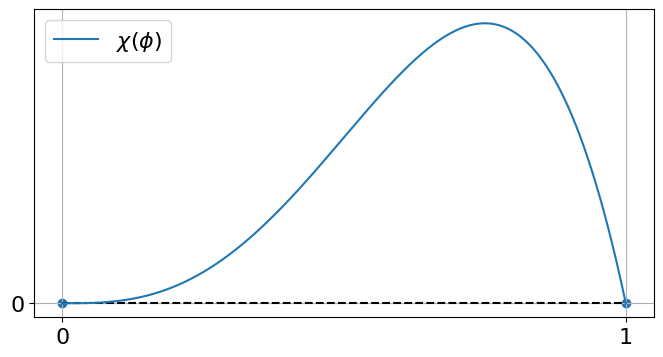
\includegraphics[width=0.84\textwidth]{figures/equilibriums_case_1.png}
  \vspace{-0.3cm}
  \caption{Characteristic behavior of~$\chi(\phi)$,
    ``weak electric field'' case.}
  \label{fig:equilibriums_case_1}
  \vspace{0.7cm}
  
  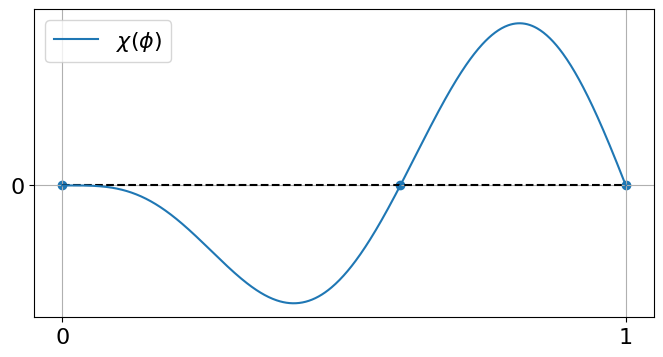
\includegraphics[width=0.84\textwidth]{figures/equilibriums_case_2.png}
  \vspace{-0.3cm}
  \caption{Characteristic behavior of~$\chi(\phi)$,
    ``medium electric field'' case.}
  \label{fig:equilibriums_case_2}
  \vspace{0.7cm}
  
  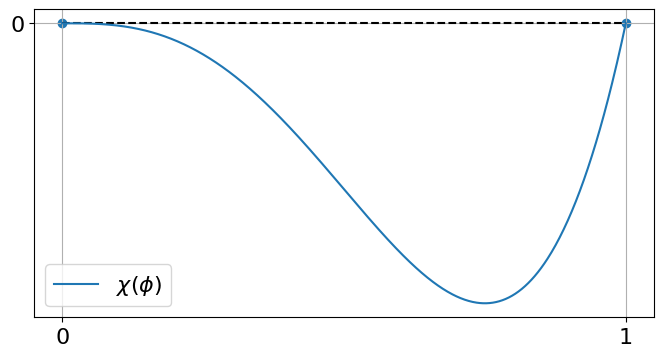
\includegraphics[width=0.84\textwidth]{figures/equilibriums_case_3.png}
  \vspace{-0.3cm}
  \caption{Characteristic behavior of~$\chi(\phi)$,
    ``strong electric field'' case.}
  \label{fig:equilibriums_case_3}
\end{figure}

% EOF